\documentclass[a4paper,11pt]{ivoa}
\usepackage[a4paper,left=1.2in,right=1.2in,top=1.2in,bottom=1.2in]{geometry}
\usepackage{lmodern}
\usepackage{natbib}
\usepackage{minted}
\usepackage{graphicx}

\title{VOEvent Transport Protocol}
\author{Alasdair Allan, Robert B. Denny, John Swinbank}
\editor{John Swinbank}
\ivoatype{IVOA Proposed Recommendadation}
\ivoagroup{Time Domain Interest Group}
\version{1.2 (draft)}


\begin{document}
\maketitle

\section*{Abstract}

The IVOA VOEvent Recommendation \citep{Seaman:2011} defines a means of
describing a transient celestial event but, purposely, remains silent on the
topic of how those descriptions should be transmitted. This document
formalizes a TCP-based protocol for VOEvent transportation that has been in
use by members of the VOEvent community for several years and discusses the
topology of the event distribution network. It is intended to act as a
reference for the production of compliant protocol implementations.

\section*{Status of this document}

This document has been produced by John Swinbank based on the version 1.1
specification by Allan \& Denny. This draft version is a work in progress. It
is intended to add clarifications to the previous version without changing the
on-the-wire protocol.

This is an IVOA Note expressing suggestions from and opinions of the authors.
It is intended to share best practices, possible approaches, or other
perspectives on interoperability with the Virtual Observatory. It should not
be referenced or otherwise interpreted as a standard specification.

A list of current IVOA Recommendations and other technical documents can be
found at \url{http://www.ivoa.net/documents/}.

\section*{Acknowledgements}

\begin{itemize}
    \item{Robert W. White, ex LANL, now at NREL}
    \item{Phillip Warner, ex NOAO}
    \item{Robert Seaman, NOAO}
\end{itemize}

Swinbank acknowledges support from the European Research Council via Advanced
Investigator Grant 247295.

\newpage

\tableofcontents

\newpage

\section{Introduction}
\label{sec:intro}

\begin{figure}
  \begin{center}
  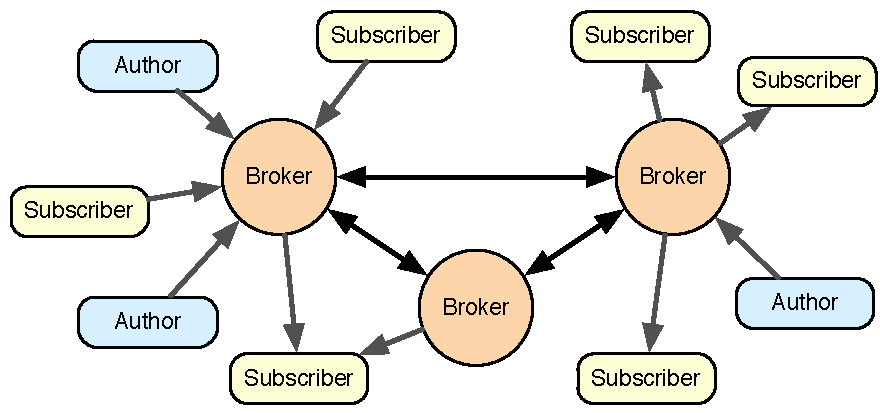
\includegraphics{figures/network.pdf}
  \end{center}

  \caption{VOEvent network architecture showing node roles.}

  \label{fig:network}
\end{figure}

The VOEvent standard \citep{Seaman:2011} defines a means of representing a
transient celestial event with an implicit request for action on the part of
the recipient. The VOEvent standard is transport neutral: it does not take a
position on the mechanism by which the event should be transmitted from its
author to interested recipients. However, it encourages the construction of
``a robust general-purpose network of interoperating brokers'' for event
transmission.

To date, a number of different event distribution networks have been
prototyped and met with varying degrees of technical success and community
adoption. However, as the number of interested participants grows, and
next-generation large-scale survey instruments such as LSST\footnote{Large
Synoptic Survey Telescope; \url{http://www.lsst.org/}}, LIGO\footnote{Laser
Interferometric Gravitational-Wave Observatory; \url{http://www.ligo.org}},
LOFAR\footnote{Low Frequency Array; \url{http://www.lofar.org}} and
SKA\footnote{Square Kilometer Array; \url{http://www.ska-telescope.org/}} are
developed and begin to become available, it is clear that a standard,
interoperable mechanism for event communication is required. It is such a
mechanism that this document aims to describe.

The purpose of the protocol described herein is to transport a VOEvent message
from its sender to one or more interested recipients. To achieve this, we
envision three distinct network roles: authors, which create events; brokers,
which receive events from authors and distribute them, and subscribers, which
receive and (if appropriate) act upon the events. See Figure \ref{fig:network}
for an illustration. Note that a single entity may perform more than one role
within the network: for example, creating events and distributing its own
creations (combining the author and broker roles) or receiving events from a
broker and redistributing them to a list of subscribers (combining the
subscriber and broker roles).

Building upon this architecture, a strongly-connected set of brokers which
subscriber to each other's event streams and redistribute to their subscribers
(the ``VOEventNet backbone'') provides a fault-tolerant system which is
resilient against the failure of one or more network entities. Such a backbone
system is already under construction by members of the VOEvent community.  The
protocol described herein is intentionally as simple as possible while still
accomplishing the required task. There are some value-added VOEvent services
being developed which may require more complex protocols, but these fall
outside the scope of the current document.

\section{Terminology}

Throughout this document, we adopt the terminology of RFC 2119
\citep{Bradner:1997}. In particular, note that:

\begin{itemize}
    \item{The word ``must'' indicates an absolute requirement of the
    specification;}

    \item{The word ``should'' indicates behavior that is normally included in
    implementations of the specification, but there may exist valid reasons
    for excluding it in particular circumstances;}

    \item{The word ``may'' indicates purely optional behavior which is
    permitted according to this specification.}
\end{itemize}

\section{Common characteristics}

\subsection{Design goals}

The Transport Protocol, hereafter VTP, is provides a simple means of
transporting VOEvents from authors through brokers to subscribers.

VTP transmits a up to single VOEvent message in each transaction. If multiple
VOEvent messages are to be transmitted, multiple transactions must take place.

VTP is non-transformational on VOEvents being transmitted: the message
delivered to a subscriber should be bit-for-bit identical to that provided by
an author. If an intermediary wishes to modify or annotate the event, they
should not edit the event in transport, but rather generate a new event to
supplement or replace it.

VTP does not provide a transport-level means of annotating or otherwise
embellishing VOEvents, or of providing stream-level metadata.

VTP values simplicity of design and operation to lower the barrier to entry. It
is not intended to meet every use case. As per Section \ref{sec:intro}, it is
anticipated that some VOEvent-based services will require more complex
protocols.

\subsection{Network layer}

VTP operates over TCP (Information Sciences Institute, 1981) connections, and
relies on TCP's guaranteed error-free in-order delivery of data: no checksum
or digest data is included. All messages are sent over the TCP connection
preceded by a 4-byte network-ordered\footnote{As defined by
\citet{Reynolds:1994}; also called ``big-endian'' ordering.} count, followed
immediately by the payload data. The 4-byte count is interpreted as a 32-bit
integer equal to the number of payload bytes following the count bytes. The
payload is considered an opaque collection of bytes at this level\footnote{As
a result, the format of the document being transmitted is opaque to the
transport layer. Therefore both ASCII and UTF-8 are equally supported}.

\subsection{Message format}
\label{sec:common:format}

The payload of the a VTP message is an XML document. It must consist of an XML
declaration followed by, in order, optional XML comments, a single VOEvent or
Transport element, and more optional XML comments. It must validate against
either the VOEvent XML
schema\footnote{\url{http://www.ivoa.net/xml/VOEvent/VOEvent-v2.0.xsd}} or the
Transport XML schema (Appendix \ref{sec:transportschema}). Transport elements
are used by the VTP system itself and are invisible to end-users: see Section
\ref{sec:transport} for details.

\subsection{Broker behaviour}

Although the simplest broker implementation may simply forward all unique
events it receives, either directly from authors or from other brokers, to all
of its subscribers, this behavior is not required. Instead, the broker may
provide ``value-added'' services which limit how messages are redistributed.
For example, a broker may make arrangements with some or all of its
subscribers to filter the events it receives, and only forward those events
fulfilling some predefined criteria to its subscribers. Similarly, brokers may
limit access to some clients based on various criteria (\S\ref{sec:limit}).

VTP does not provide in-band notification of these per-broker details. For
example, the protocol does not make an author submitting to a filtering broker
aware that their event might not be sent to all of the broker's subscribers,
and, similarly, it does not make a subscriber of a filtering broker aware that
they might not receive a complete set of events. It is the responsibility of
authors and subscribers to ensure that the brokers they use provide the
services they require. Brokers should clearly advertise any added-value
behavior they provide, for example on a website or through the IVOA registry.

\section{Node roles}
\label{sec:noderoles}

The VOEvent network consists of three types of nodes (refer to Fig.
\ref{fig:network}):

\begin{itemize}
    \item{Author}
    \item{Broker}
    \item{Subscriber}
\end{itemize}

The flow of messages is over three types of connections:

\begin{itemize}
    \item{Author to Broker}
    \item{Broker to Subscriber}
    \item{Broker to Broker}
\end{itemize}

Each type of connection is discussed qualitatively below.

\subsection{Author to Broker}

When an author wants to submit a VOEvent message to the network, it opens a
TCP connection to a broker, sends the message, waits for a response from the
broker, and then closes the TCP connection. The response from the broker is a
Transport message.

\subsection{Broker to Subscriber}

When a subscriber wants to receive VOEvent message traffic, it opens a TCP
connection to a broker. This connection is kept open continuously. When the
broker receives a message, it relays a copy of the VOEvent message to all of
the connected subscribers. Thus, a subscriber must continuously listen on the
TCP connection and be prepared to receive VOEvent messages at any time, even
when it is busy processing a previously received VOEvent message. When a
subscriber receives a VOEvent message from its broker, it must respond with an
appropriate Transport message.

\subsection{Broker to Broker}
\label{sec:node:brokertobroker}

Traffic between brokers uses the preceding methods. Each broker takes the role
subscriber as far as every other broker is concerned. A broker that wishes to
receive a feed from another broker should connect to that broker's subscriber
port. No special protocol features are needed.

\section{Connection Maintenance}
\label{sec:maintenance}

All connections over which a broker sends VOEvent messages are kept open
continuously. Basic TCP does not provide any dead-peer indication\footnote{
TCP does support a ``keep-alive'' service, but it is not universally available
\citep{Braden:1989}.}. Further, network infrastructure devices might sever a
TCP connection after some period of inactivity. This gives rise to the need
for keep-alive messages. After no more than 90 seconds of inactivity on any
given connection, the broker must send a Transport \texttt{iamalive} message,
to which the subscriber must reply with a copy of that message plus some
optional identification information. For details of the message format, see
Section \ref{sec:transport}.  At both ends of the continuous connection, the
node either expects to receive an \texttt{iamalive} message or expects to
receive the response to its \texttt{iamalive} message. If not seen, the node
should assume that the connection has been lost or the peer is dead. At this
point, the node that was responsible for opening the connection may attempt to
re-initiate it. A geometric back-off algorithm may be used to avoid network
load.

\section{Transport messages}
\label{sec:transport}

Transport messages are XML documents. There are four classes of Transport
message:

\begin{itemize}
\item{\texttt{iamalive} (Connection maintenance);}
\item{\texttt{authenticate} (Authentication request/response);}
\item{\texttt{ack} (VOEvent successful receipt acknowledgement);}
\item{\texttt{nak} (VOEvent unsuccessful receipt acknowledgement).}
\end{itemize}

All Transport messages have the same general syntax, and are defined by the
Transport schema (Appendix \ref{sec:transportschema}). The \texttt{role}
attribute of the root \texttt{<Transport>} element distinguishes between the
types listed above. The connection maintenance and receipt acknowledgement
message types are described in detail in this section; the authentication
message type has a special role which is described in Section
\ref{sec:limit:crypto:subscriber}.

\subsection{\texttt{iamalive} message}
\label{sec:transport:iamalive}

The \texttt{iamalive} message is indicated by a role equal to
\texttt{iamalive}. The \texttt{<Origin>} element contains the
IVORN\footnote{International Virtual Observatory Resource Name
\citep{Plante:2007}.} of the broker which is managing the connection.  The
\texttt{<TimeStamp>} element must contain the UTC date/time at which the
message was generated.

\begin{listing*}
\begin{minted}[fontsize=\small,frame=lines]{xml}
<?xml version="1.0" encoding="UTF-8"?>

<trn:Transport role="iamalive" version="1.0"
 xmlns:trn="http://telescope-networks.org/schema/Transport/v1.1"
 xmlns:xsi="http://www.w3.org/2001/XMLSchema-instance"
 xsi:schemaLocation="http://telescope-networks.org/schema/Transport/v1.1
                     http://telescope-networks.org/schema/Transport-v1.1.xsd">
    <Origin>ivo://uk.org.estar/estar.ex#</Origin>
    <TimeStamp>2009-04-09T22:39:06</TimeStamp>
</trn:Transport>
\end{minted}
\caption{Sample \texttt{iamalive} message.}
\label{lst:iamalive}
\end{listing*}

\subsection{\texttt{iamalive} response}
\label{sec:transport:iamaliveresponse}

The \texttt{iamalive} response is an extension of the initial iamalive
message. It also has a role of \texttt{iamalive}. It must include an
additional \texttt{<Response>} element containing the IVORN of the subscriber.
It may include a \texttt{<Meta>} element with \texttt{<Param>} sub-elements
which give additional information about the subscriber or any other relevant
information. \texttt{<Param>} elements have no content and must contain name
and value attributes. The names and values may be any string. The
\texttt{<TimeStamp>} element contains the UTC date and time at which the
response is sent.

\begin{listing*}
\begin{minted}[fontsize=\small,frame=lines]{xml}
<?xml version='1.0' encoding='UTF-8'?>

<trn:Transport role="iamalive" version="1.0"
 xmlns:trn="http://telescope-networks.org/schema/Transport/v1.1"
 xmlns:xsi="http://www.w3.org/2001/XMLSchema-instance"
 xsi:schemaLocation="http://telescope-networks.org/schema/Transport/v1.1
                     http://telescope-networks.org/schema/Transport-v1.1.xsd">
    <Origin>ivo://uk.org.estar/estar.ex#</Origin>
    <Response>ivo://com.dc3/engineering#</Response>
    <TimeStamp>2009-04-09T22:39:07</TimeStamp>
    <Meta>
        <Param name="IPAddr" value="123.123.123.123" />
        <Param name="Contact" value="rdenny@dc3.com" />
    </Meta>
</trn:Transport>
\end{minted}
\caption{Sample \texttt{iamalive} response.}
\label{lst:iamaliveresponse}
\end{listing*}

\subsection{VOEvent message receipt response}
\label{sec:transport:ack}

The VOEvent message receipt response is similar to the \texttt{iamalive}
response except the role is either \texttt{ack} or \texttt{nak}, the
\texttt{<Origin>} is the IVORN of the just-received VOEvent message, and an
optional \texttt{<Result>} element may accompany the \texttt{<Param>}
elements. \texttt{<Result>} may contain any string; it is recommended that it
contain a human-readable error message if role is \texttt{nak}. The
\texttt{<TimeStamp>} element contains the UTC date and time at which the
response is sent.

The \texttt{nak} response indicates that the recipient is unable or unwilling
to take responsibility for this message. This may be because, for example, the
message fails to validate as a valid VOEvent, or because it was received from
an unauthorized client (\S\ref{sec:limit}). A \texttt{nak} response is not
appropriate if the sender is able to accept the message but then decides not
to redistribute it (for example, if it is a duplicate of an event which has
already been distributed: Section \ref{sec:dedup}).

\begin{listing*}
\begin{minted}[fontsize=\small,frame=lines]{xml}
<?xml version='1.0' encoding='UTF-8'?>

<trn:Transport role="ack" version="1.0"
 xmlns:trn="http://telescope-networks.org/schema/Transport/v1.1"
 xmlns:xsi="http://www.w3.org/2001/XMLSchema-instance"
 xsi:schemaLocation="http://telescope-networks.org/schema/Transport/v1.1
                     http://telescope-networks.org/schema/Transport-v1.1.xsd">
    <Origin>ivo://nvo.caltech/voeventnet/catot#901211380084129246</Origin>
    <Response>ivo://com.dc3/engineering#</Response>
    <TimeStamp>2009-04-09T22:54:01</TimeStamp>
    <Meta>
        <Param name="IPAddr" value="123.123.123.123" />
        <Param name="Contact" value="rdenny@dc3.com" />
        <Result>Message received and validated successfully</Result>
    </Meta>
</trn:Transport>
\end{minted}
\caption{Sample VOEvent message receipt response indicating successful
transmission (\texttt{ack}).}
\label{lst:ack}
\end{listing*}

\begin{listing*}
\begin{minted}[fontsize=\small,frame=lines]{xml}
<?xml version='1.0' encoding='UTF-8'?>

<trn:Transport role="nak" version="1.0"
 xmlns:trn="http://telescope-networks.org/schema/Transport/v1.1"
 xmlns:xsi="http://www.w3.org/2001/XMLSchema-instance"
 xsi:schemaLocation="http://telescope-networks.org/schema/Transport/v1.1
                     http://telescope-networks.org/schema/Transport-v1.1.xsd">
    <Origin>ivo://nvo.caltech/voeventnet/catot#901211380084129246</Origin>
    <Response>ivo://com.dc3/engineering#</Response>
    <TimeStamp>2009-04-09T22:54:01</TimeStamp>
    <Meta>
        <Param name="IPAddr" value="123.123.123.123" />
        <Param name="Contact" value="rdenny@dc3.com" />
        <Result>Error in VOEvent message: ISOTime not in ISO 8601 format</Result>
    </Meta>
</trn:Transport>
\end{minted}
\caption{Sample VOEvent message receipt response indicating unsuccessful
transmission (\texttt{nak}).}
\label{lst:nak}
\end{listing*}

\section{Protocol operation}

\begin{figure}
  \begin{center}
  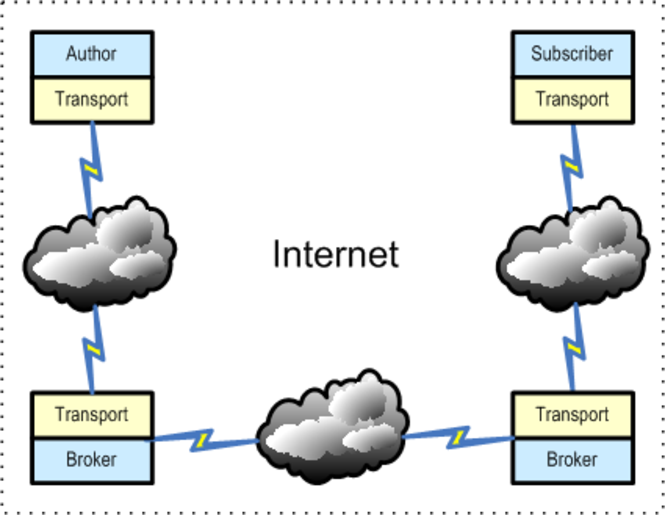
\includegraphics{figures/architecture.pdf}
  \end{center}

  \caption{Layered architecture.}

  \label{fig:architecture}
\end{figure}

This section describes the operation and sequencing of VTP operation for each
end of a connection between an author and a broker, as well as between a
broker and a subscriber. See Section \ref{sec:noderoles} above for a
qualitative discussion of the protocol from the viewpoint of each entity. In
the sections below, the ``message'' is the combination of the byte count and
payload as described in Section \ref{sec:common:format} above.

The protocol diagrams in the following sections depict layers between which
are interfaces. Figure \ref{fig:architecture} shows the overall architecture
of communication between authors, brokers, and subscribers. Each entity uses
the transport layer to send and/or receive VOEvent messages.

\subsection{Author sending to broker}

\begin{figure}
  \begin{center}
  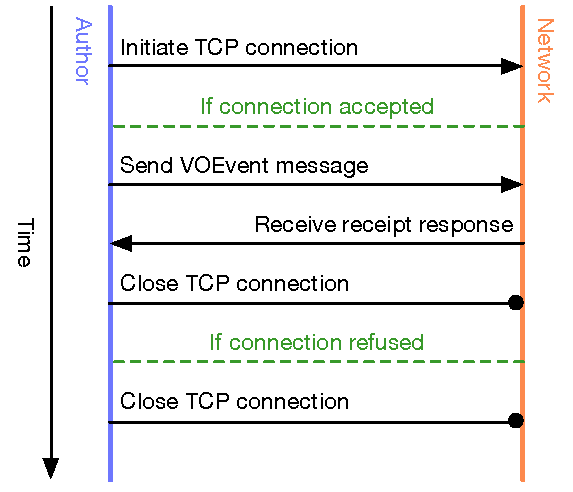
\includegraphics{figures/authortobroker.pdf}
  \end{center}

  \caption{Transport protocol at an author node.}

  \label{fig:protocol:authortobroker}
\end{figure}


The author provides a single, complete event to the transport layer for
transmission. It is the responsibility of the author to apply a digital
signature (\S\ref{sec:limit:crypto}) to the message if required before sending
it to the transport layer. It is the responsibility of the transport layer to
prepend the byte count (\S\ref{sec:common:format}) to the message before
sending it to the broker, and to interpret the \texttt{ack} or \texttt{nak}
response from the broker (\S\ref{sec:transport:ack}).  The transport layer
returns a value indicating success or failure to the author; it is the
responsibility of the author to check this and to initiate any appropriate
responsive action. See Figure \ref{fig:protocol:authortobroker} for details.

\subsection{Broker receiving from author}

\begin{figure}
  \begin{center}
  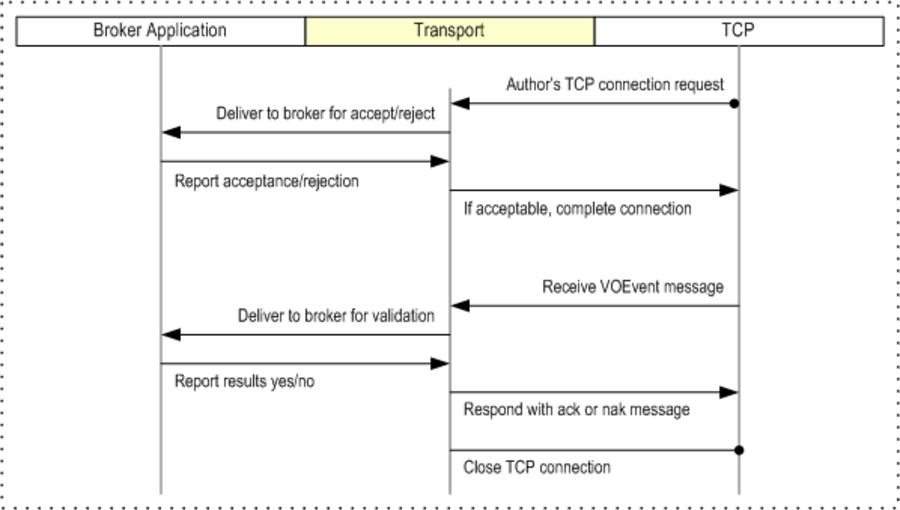
\includegraphics{figures/brokerfromauthor.pdf}
  \end{center}

  \caption{Transport protocol at broker receiving from author.}

  \label{fig:protocol:brokerfromauthor}
\end{figure}

The broker responds to two events from the transport layer, as shown in Figure
\ref{fig:protocol:brokerfromauthor}. One event indicates that a request for a
TCP connection has arrived, and the broker must respond with accept or reject
status. This is where the broker can provide IP whitelist access control
(\S\ref{sec:limit:whitelist}). The other event indicates that a message has
been received, and the broker must respond with accept or reject status. This
is where the broker can validate the XML and check any digital signature
(\S\ref{sec:limit:crypto:author}). It is the responsibility of the Transport
layer to remove the byte count (\S\ref{sec:common:format}) from the incoming
message, and to create the \texttt{ack} or \texttt{nak} response
(\S\ref{sec:transport:ack}).

\subsection{Broker sending to subscriber}

\begin{figure}
  \begin{center}
  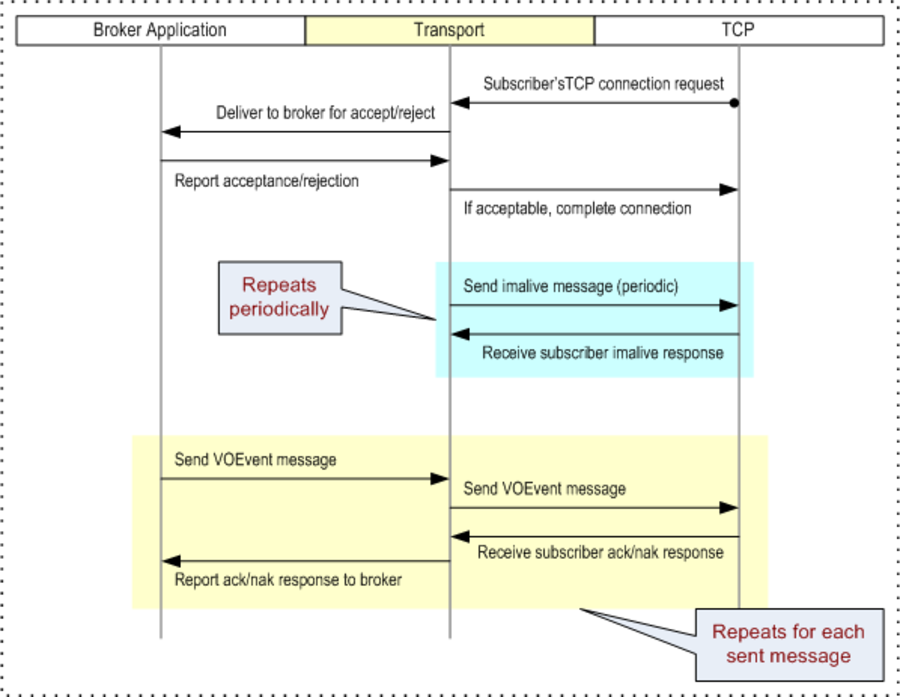
\includegraphics{figures/brokertosub.pdf}
  \end{center}

  \caption{Transport protocol at broker sending to subscriber.}

  \label{fig:protocol:brokertosub}
\end{figure}

See Figure \ref{fig:protocol:brokertosub}. Subscribers connect to the broker
and leave the connection open indefinitely. The broker responds to an event
from the transport layer indicating that a subscriber wants to open a TCP
connection, and the broker must respond with accept or reject status. This is
where the broker can provide IP white list access control
(\S\ref{sec:limit:whitelist}). If accepted, the broker would presumably add
this subscriber to its distribution list.

Once the subscriber has successfully connected to the broker, the broker's
Transport layer begins sending periodic \texttt{iamalive} messages to the
subscriber, which replies with an \texttt{iamalive} response
(\S\S\ref{sec:transport:iamalive} and \ref{sec:transport:iamaliveresponse}).
If the subscriber's \texttt{iamalive} reply messages stop arriving, the
Transport layer may assume that the subscriber is dead or gone, and close the
TCP connection. The \texttt{iamalive} exchange continues until the subscriber
closes the TCP connection or the broker's Transport layer stops receiving
\texttt{iamalive} replies from the subscriber.

To send a message to the subscriber, the broker provides it to the Transport
layer. It is the responsibility of the transport layer to prepend the byte
count (\S\ref{sec:common:format}) to the message before sending to the
subscriber, and to interpret the resulting \texttt{ack} or \texttt{nak}
message (\S\ref{sec:transport:ack}). The Transport layer returns a value
indicating success or failure to the broker; in the event of an error
(\texttt{nak} received, dead-peer, or subscriber closed the connection), the
broker may remove the subscriber from its distribution list.

\subsection{Subscriber receiving from broker}

\begin{figure}
  \begin{center}
  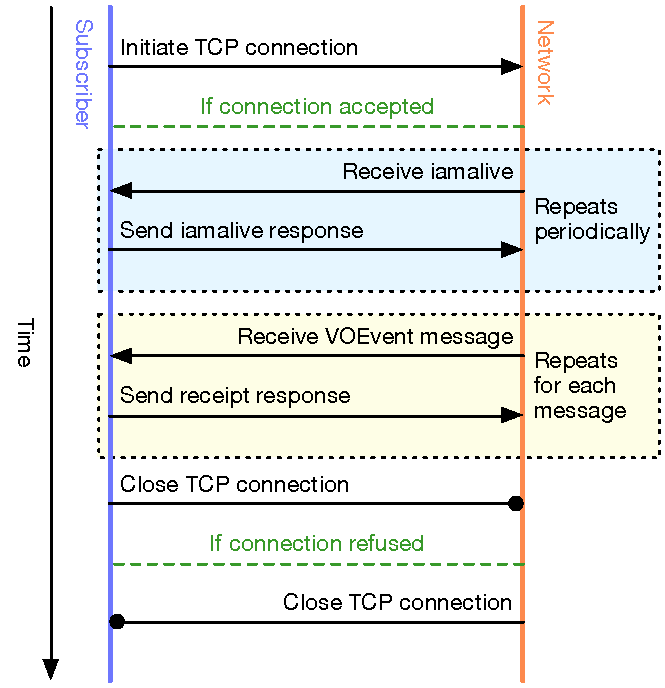
\includegraphics{figures/subfrombroker.pdf}
  \end{center}

  \caption{Transport protocol at subscriber.}

  \label{fig:protocol:subfrombroker}
\end{figure}

See Figure \ref{fig:protocol:subfrombroker}. Subscribers connect to the broker
and leave the connection open indefinitely. If the connection is successful,
the subscriber will begin receiving messages.

As per Section \ref{sec:maintenance}, when the subscriber has successfully connected to the
broker, the subscriber's Transport layer begins listening for periodic
\texttt{iamalive} (\S\ref{sec:transport:iamalive}) messages from the broker.
For each \texttt{iamalive} message
received, the Transport layer responds with an \texttt{iamalive} response
(\S\ref{sec:transport:iamaliveresponse}).
If the broker's iamalive messages stop arriving, the subscriber's Transport
layer may assume that the connection has been lost and attempt to re-connect
to the broker. Reconnection attempts should use ageometric back-off algorithm.
If the subscriber's Transport layer cannot re-establish the connection, it
should notify the subscriber of the error.

The subscriber client responds to an event advising that a (VOEvent) message
has arrived, and the subscriber client must respond with accept or reject
status. This is where the subscriber can validate the XML and check any
digital signature that may be present. It is the responsibility of the
Transport layer to remove the byte count (\S\ref{sec:common:format}) from the
incoming message, and to create and send the \texttt{ack} or \texttt{nak}
message (\S{sec:transport:ack}).

\section{De-duplication}
\label{sec:dedup}

In a network topology like that illustrated in Figure \ref{fig:network},
multiple brokers service independent sets of authors and subscribers. As per
Sections \ref{sec:intro} and \ref{sec:node:brokertobroker}, brokers will
subscribe to each other's event feeds to ensure that their subscribers have
access to the full range of available events. In this way, in a complex
VOEvent network, many brokers will form one or more strongly connected sets.

In this situation, there is a risk of event loops developing on the network:
broker A receives an event from B and forwards it to its subscriber list,
which includes A, which forwards it to its subscriber lists, which includes B,
and so on.

In order to prevent this, each broker must process each unique event it
receives a maximum of once. For this purpose, we regard ``unique'' as meaning
that the content between the opening \texttt{<} and closing \texttt{>} of the
\texttt{<VOEvent>} element is bit-for-bit identical, including all white space
characters\footnote{The implementation of this check is at the discretion of
the broker. Appropriate techniques may include directly comparing the
bitstream (which would necessarily mean storing an archive of
previously-processed events) or calculating a hash function such as SHA1
\citep{Eastlake:2001} over the event contents and storing the result.}. Note
that it is now established practice to distribute different serializations
(e.g.  VOEvent 1.1 and 2.0) of the same event with the same
IVORN\footnote{\url{http://www.ivoa.net/pipermail/voevent/2012-March/002836.html}
and subsequent discussion.}.  Consequently, an IVORN is not a unique
identifier of a particular event representation, and is not, therefore,
suitable for use in network de-duplication.

\section{Limiting access}
\label{sec:limit}

\subsection{IP address whitelisting}
\label{sec:limit:whitelist}

\subsection{Cryptographic signatures}
\label{sec:limit:crypto}

\subsubsection{Author submission}
\label{sec:limit:crypto:author}

\subsubsection{Subscriber authentication}
\label{sec:limit:crypto:subscriber}

\appendix

\section{Transport schema}
\label{sec:transportschema}

\bibliographystyle{elsarticle-harv}
\bibliography{vtp}

\end{document}
